\documentclass[11pt]{article}
\usepackage[T1]{fontenc}
\usepackage[latin9]{inputenc}
\usepackage{textcomp}
\usepackage{amstext}
\usepackage{graphicx}
\usepackage{amssymb}
\makeatletter
\providecommand{\tabularnewline}{\\}
\usepackage{mdwlist}
\usepackage{fourier-orns}
\usepackage[colorlinks,linkcolor=blue]{hyperref}
\usepackage{footmisc}
\usepackage{subfigure}
\usepackage{float}

\topmargin=-0.7in
\oddsidemargin = -0.2in
\parindent=0.0cm
\parskip=0.3cm
\textwidth=6.9in
\textheight= 9.8in

\sloppy
\newtheorem{theorem}{Theorem}[section]
\newtheorem{lemma}{Lemma}[section]
\newtheorem{corollary}{Corollary}[section]
\newtheorem{definition}{Definition}[section]


\begin{document}
\pagestyle{empty}

{\bf What benefits/problems come from deploying services in Serverless functions?}

Benefits:
\begin{itemize*}
  \item {\bf Improve develop efficiency:} Serverless computing does not mean developers work without any server. It instead allows them not to focus on issues related to server-based architectures. Therefore, developers can pay more attention to the logic for processing client requests, which can improve efficiency of software development. 
  \item {\bf Decrease develop cost:} Past IDC and modern cloud architecture, which normally uses a monthly charging mode, can result in the situation that they still charge even if no current users or no applications are deployed. Contrastingly, Serverless architecture often uses a Pay-as-you-go mode, which allows only paying infrastructure provider for resources they actually used, and not pay for idle capacity. For example, with AWS\footnote{https://aws.amazon.com/pricing/} developers pay only for the individual services, for as long as using periods, and without requiring long-term contracts or complex licensing, which have a potential savings range from 99.8\% to 99.95\%\cite{no1}. 
  \item {\bf Reduction in lead time:} Packaging and deploying a Serverless function are simple compared to deploying an entire server. All server-related works that used to be allocated to architects are handed to infrastructure provider, which is fast, and saves workforce. A fully Serverless solution requires zero system administration. For example, no Puppet/Chef, no start/stop shell scripts, and no decisions about whether to deploy one or many containers on a machine\cite{no2}. Easier operational management makes it use less time to market. 
\end{itemize*}
Problems:
\begin{itemize*}
  \item {\bf Startup latency:} Empirical evidence suggests Serverless architecture usually do long time preparation before going into runtime. The latency introduced by multiple hops, and tail-effects also need to be taken into consideration\cite{no1}, as rapidly increasing number of request will result in time out. AWS has improved this area over time, but there are still significant concerns.
  \item {\bf Hard to debug:} It is difficult to troublesome problems because implementation logic is almost everywhere and a simple operation may cause thousands of Lambdas to execute. There has been some progress, mostly related to running functions locally, or in line with the testing updates. AWS X-Ray\footnote{https://aws.amazon.com/xray/} and CloudWatch\footnote{https://aws.amazon.com/cloudwatch/} can help developers monitering and managing. 
  \item {\bf Restrictions from vendors:} Serverless increase market monopoly that was already severe in Cloud architecture. As our Serverless features are proveded by third-party vendors, restrictions from vendors are inevitable. For example, lack of system control may manifest as system downtime, unexpected limits, cost changes, loss of functionality, forced API upgrades, etc.\cite{no2}
\end{itemize*}
We can learn from a case study from MindMup (a commercial online mind-mapping application) to see the cost saving benefits of Serverless. Between February 2016 (running on Heroku) and February 2017 (running on Lambda), the number of active users supported by the platform grew by more than 50\%, but the hosting costs dropped by slightly less than 50\%\cite{no1}. 

{\footnotesize
\begin{thebibliography}{9}
    \bibitem{no1}
    A. Colyer, \textbf{Serverless computing: economic and architectural impact}
    \url{https://blog.acolyer.org/2017/10/19/Serverless-computing-economic-and-architectural-impact/}
    \textit{Date Accessed: 21 February 2019}
    
    \bibitem{no2}
    M. Roberts, \textbf{Serverless Architectures}
    \url{https://martinfowler.com/articles/Serverless.html}
    \textit{Date Accessed: 22 February 2019}
\end{thebibliography}
}


{\bf Part II: }\\[10px]
% \section{diagram}
  
            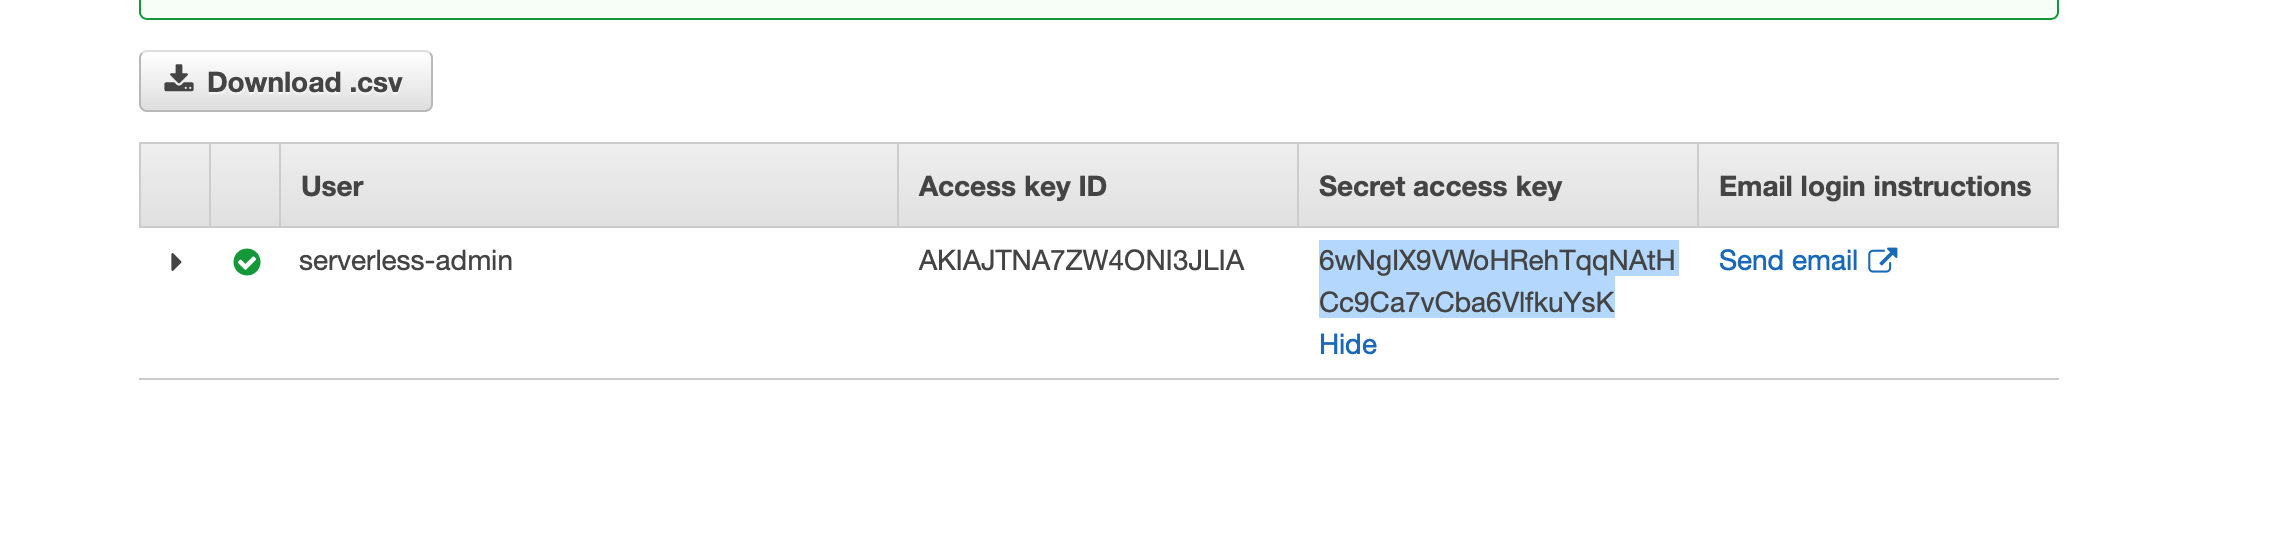
\includegraphics[width=\textwidth,height = 4cm ]{keys.png}
            this is the image that we get the secret key and access ID \\
            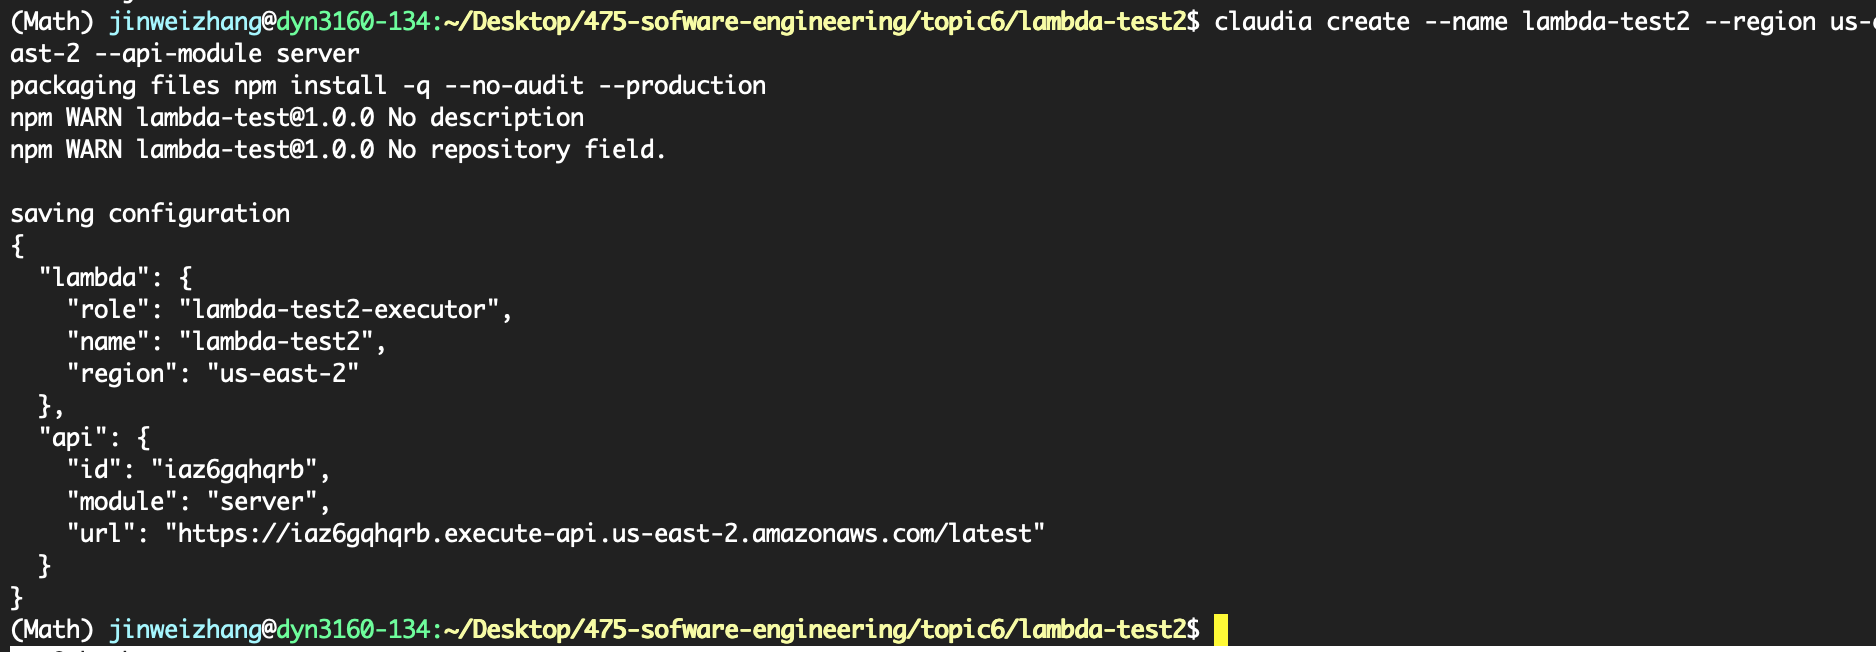
\includegraphics[width=\textwidth,height = 4cm ]{deploy.png}
            this is the json file that shows up when we succeed in deploying the application onto amazon aws
            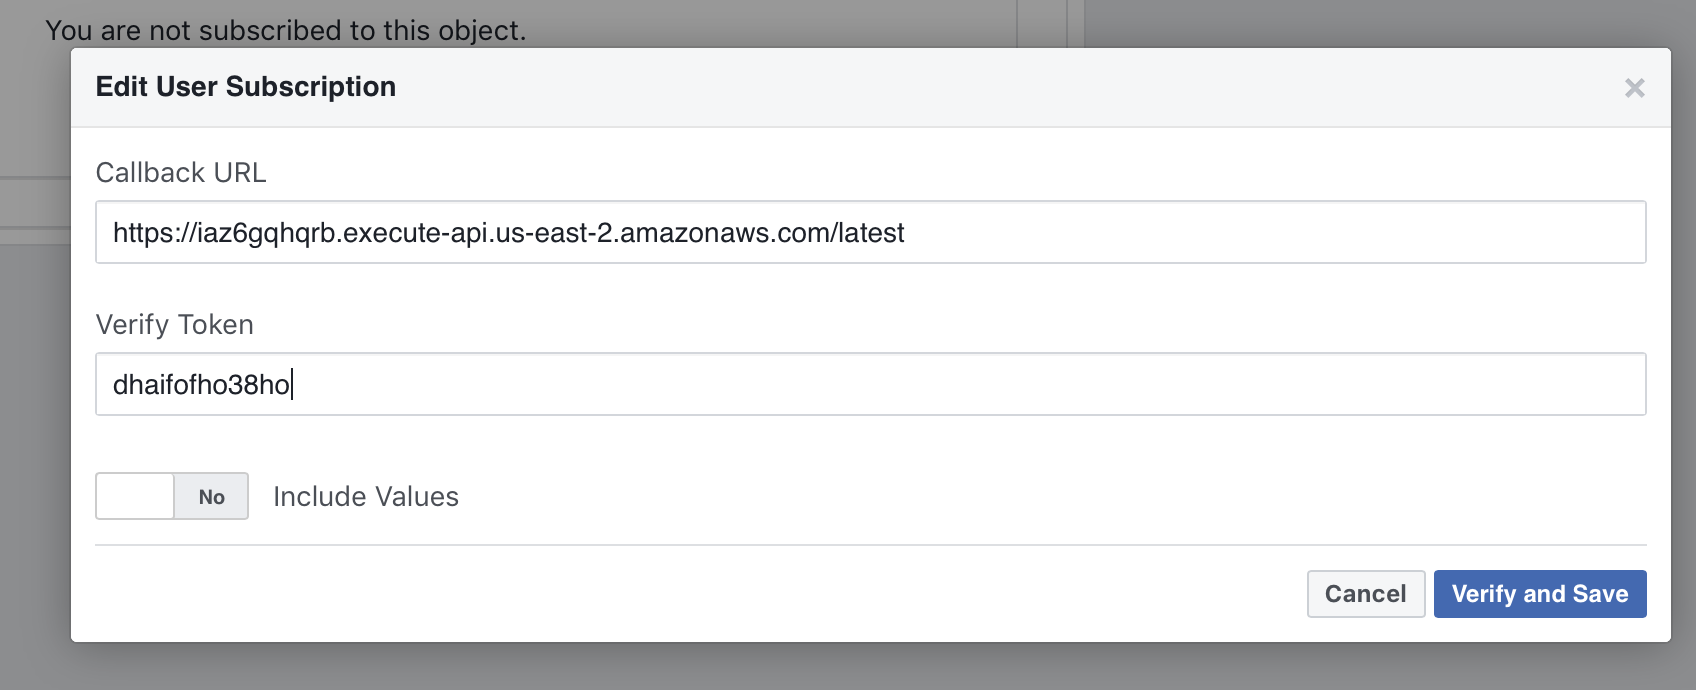
\includegraphics[width=\textwidth,height = 4cm ]{t.png}
            
            this is the page callback URL and token \\
            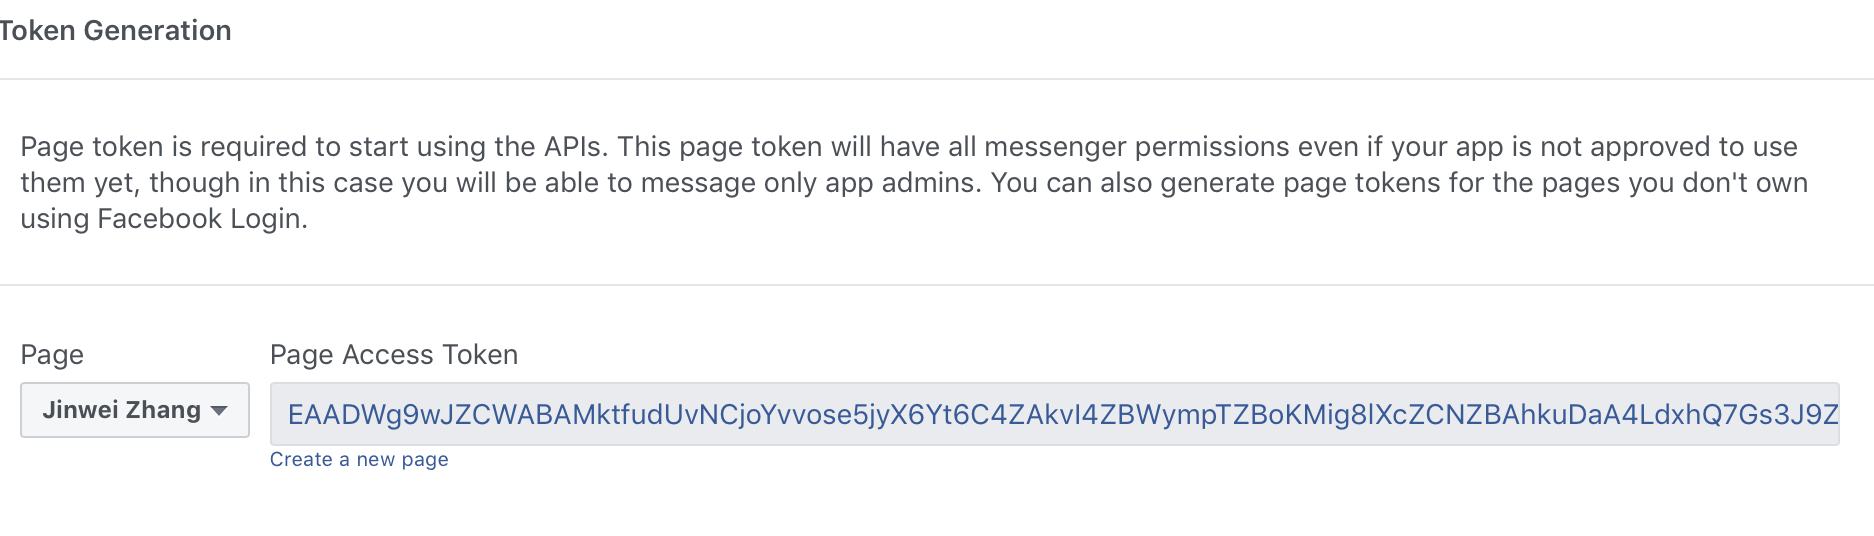
\includegraphics[width=\textwidth,height = 3cm ]{t2.png}
            
            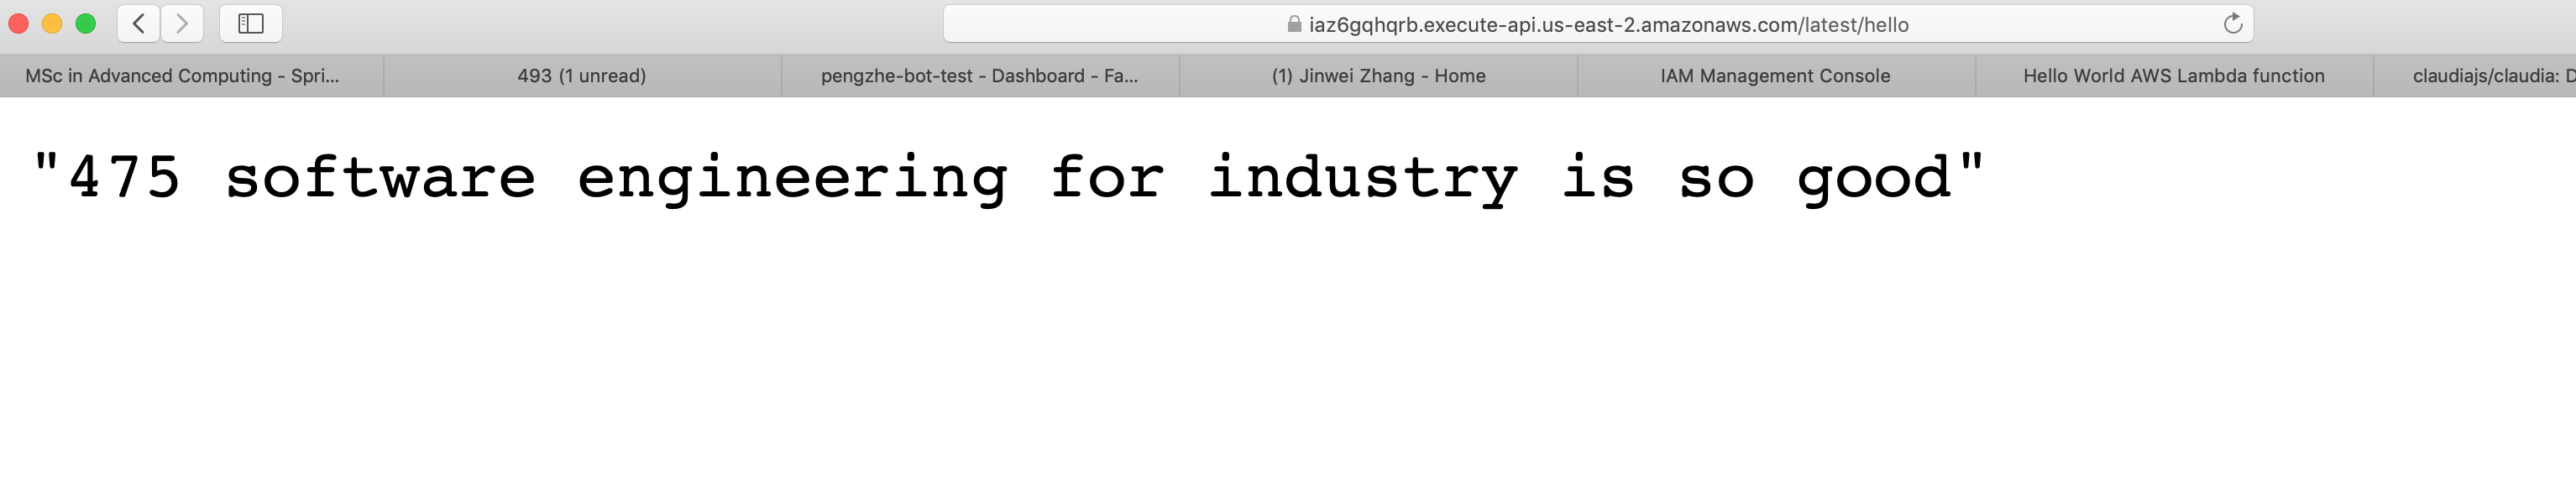
\includegraphics[width=\textwidth,height = 4cm ]{res.png}
            
            a simple sentence that called from server. 
  
        

\end{document}